%%%%%%%%%%%%%%%%%%%%%%%%%%%%%%%%%%%%%%%%%%%%%%%%%%%%%%%%%%%%%%%%%%%%%%
% Overleaf (WriteLaTeX) Example: Molecular Chemistry Presentation
%
% Source: http://www.overleaf.com
%
% In these slides we show how Overleaf can be used with standard 
% chemistry packages to easily create professional presentations.
% 
% Feel free to distribute this example, but please keep the referral
% to overleaf.com
% 
%%%%%%%%%%%%%%%%%%%%%%%%%%%%%%%%%%%%%%%%%%%%%%%%%%%%%%%%%%%%%%%%%%%%%%

\documentclass{beamer}

\mode<presentation>
{
  \usetheme{Madrid}       % or try default, Darmstadt, Warsaw, ...
  \usecolortheme{default} % or try albatross, beaver, crane, ...
  \usefonttheme{default}    % or try default, structurebold, ...
  \setbeamertemplate{navigation symbols}{}
  \setbeamertemplate{caption}[numbered]
} 

\usepackage[english]{babel}
\usepackage[utf8x]{inputenc}
\usepackage{graphicx}
\usepackage{hyperref}
  \hypersetup{colorlinks=true}
  \hypersetup{urlcolor=blue}
  \hypersetup{linkcolor = .}
\usepackage{xcolor}
\usepackage{siunitx}
  \sisetup{separate-uncertainty = true}
\usepackage{physics}
\usepackage[font=small,labelfont=bf]{caption}
\usepackage{subcaption}
\usepackage[en-GB]{datetime2}
\usepackage{overpic}
\usepackage{feynmp}
\DeclareGraphicsRule{*}{mps}{*}{}
\usepackage{scalerel}
\newcommand{\mylbrace}[2]{\vspace{#2pt}\hspace{6pt}\scaleleftright[\dimexpr5pt+#1\dimexpr0.06pt]{\lbrace}{\rule[\dimexpr2pt-#1\dimexpr0.5pt]{-4pt}{#1pt}}{.}}
\newcommand{\myrbrace}[2]{\vspace{#2pt}\scaleleftright[\dimexpr5pt+#1\dimexpr0.06pt]{.}{\rule[\dimexpr2pt-#1\dimexpr0.5pt]{-4pt}{#1pt}}{\rbrace}\hspace{6pt}}

% Trim in percent
\usepackage{adjustbox}

% No "Figure" prefix
\setbeamertemplate{caption}{\raggedright\insertcaption\par}

\usepackage{amsmath,amssymb,tikz-cd}

% Here's where the presentation starts, with the info for the title slide
\title[$B^\pm\to(K^+K^-\pi^+\pi^-)_Dh^\pm$]{Model-independent determination of the CKM angle \texorpdfstring{$\gamma$}{gamma} in \texorpdfstring{$B^\pm\to(K^+K^-\pi^+\pi^-)_Dh^\pm$}{B to K+K-pi+pi-} decays}

\author{Martin Tat}
\institute[University of Oxford]{\normalsize University of Oxford\\ \vspace{0.3cm}\normalsize Warwick EPP Seminar}
\date{9th Februrary 2023}

\titlegraphic{
\includegraphics[height = 2cm]{lhcb.jpg}\hspace{2cm}~%
              
\includegraphics[height = 2cm]{OxfordLogo.pdf}}

\begin{document}

\begin{frame}
  \titlepage
\end{frame}

% These three lines create an automatically generated table of contents.
% \begin{frame}{Outline}
%   \tableofcontents
% \end{frame}

\section{Introduction to \texorpdfstring{$C\!P$}{CP} violation}
\begin{frame}{Introduction to $C\!P$ violation}
  \begin{center}
    {\huge Introduction to $C\!P$ violation}
  \end{center}
\end{frame}

\begin{frame}{Big Bang and matter-antimatter asymmetry}
  \begin{figure}
    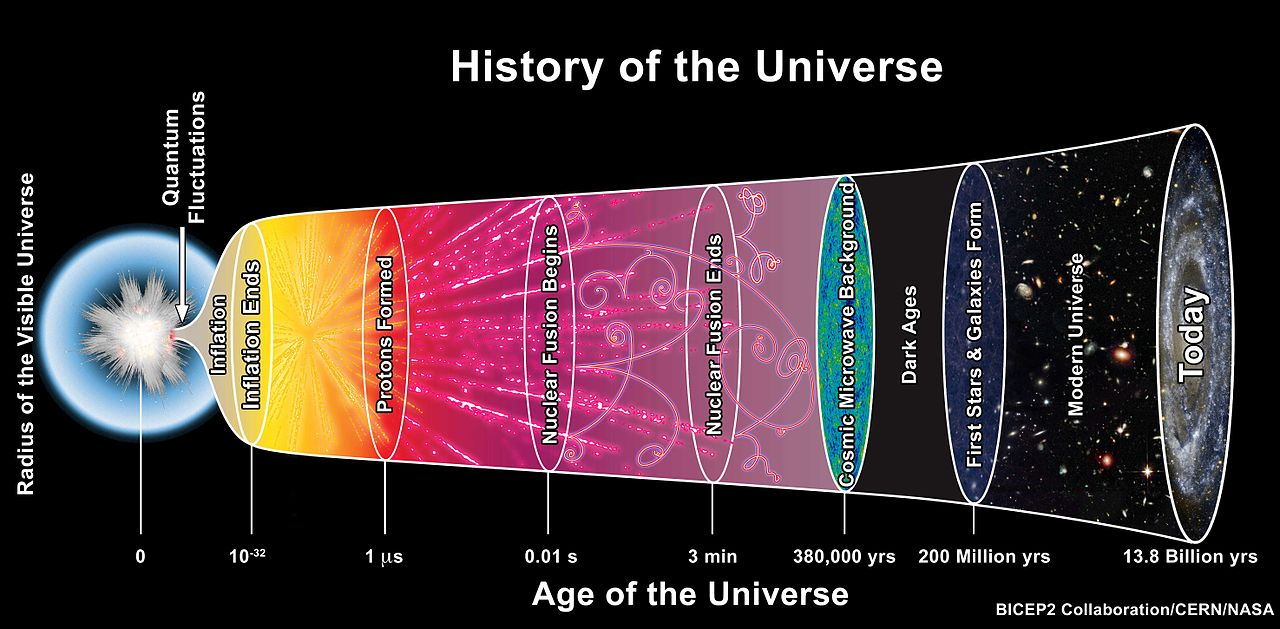
\includegraphics[height=5.5cm]{Plots/BigBangHistory.jpg}
  \end{figure}
  \begin{center}
    \Large Where is the antimatter in the universe?
  \end{center}
\end{frame}

\begin{frame}{Big Bang and matter-antimatter asymmetry}
  \begin{figure}
    \adjustbox{trim={0} {0} {0.838\width} {0},clip=true}{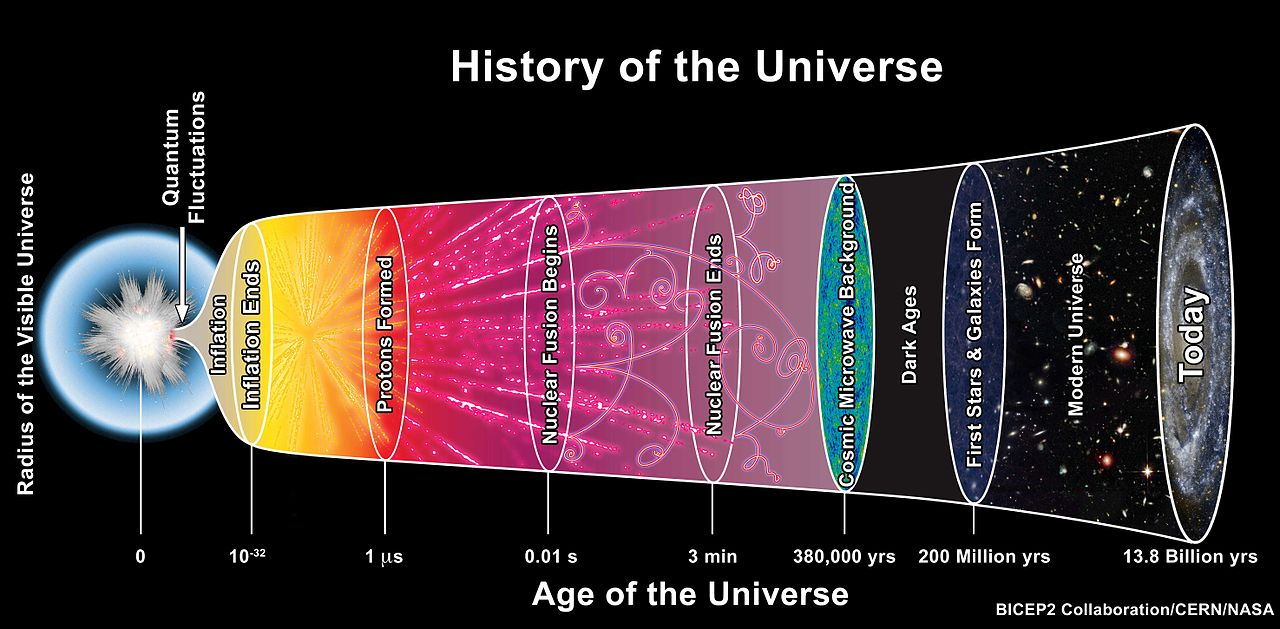
\includegraphics[height=5.5cm]{Plots/BigBangHistory.jpg}}%
    \adjustbox{trim={0.162\width} {0} {0} {0},clip=true}{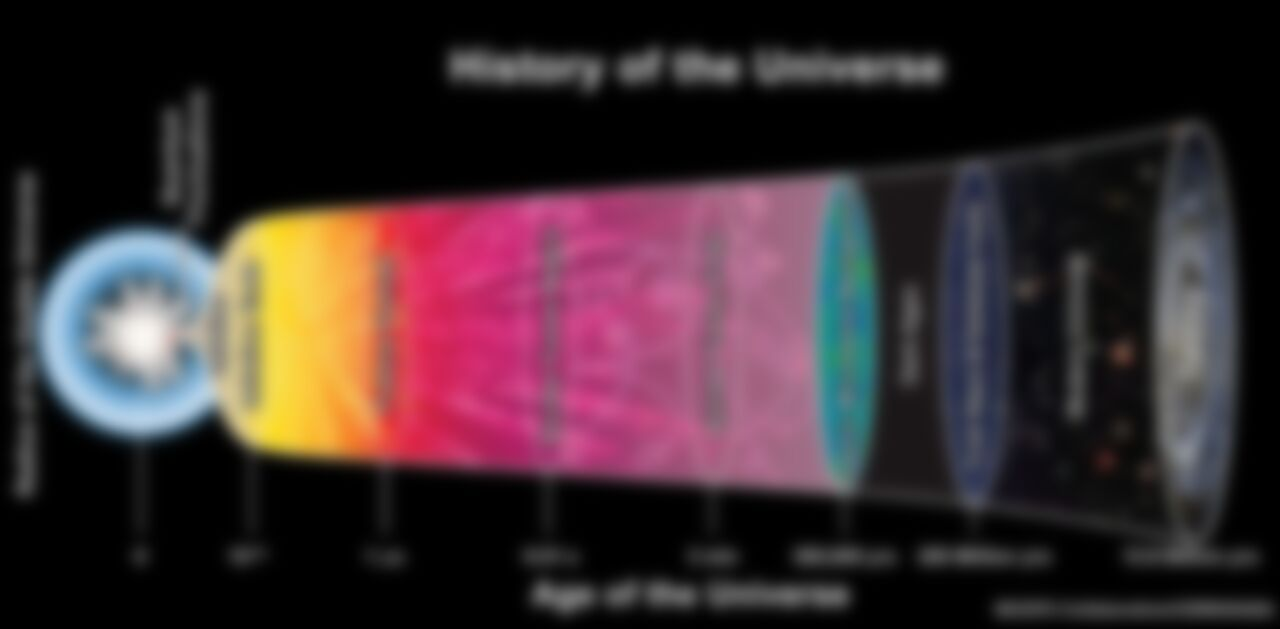
\includegraphics[height=5.5cm]{Plots/BigBangHistory_blur.jpg}}
  \end{figure}
  \begin{center}
    \Large Initially equal amounts of matter and antimatter...
  \end{center}
\end{frame}

\begin{frame}{Big Bang and matter-antimatter asymmetry}
  \begin{figure}
    \adjustbox{trim={0} {0} {0.18\width} {0},clip=true}{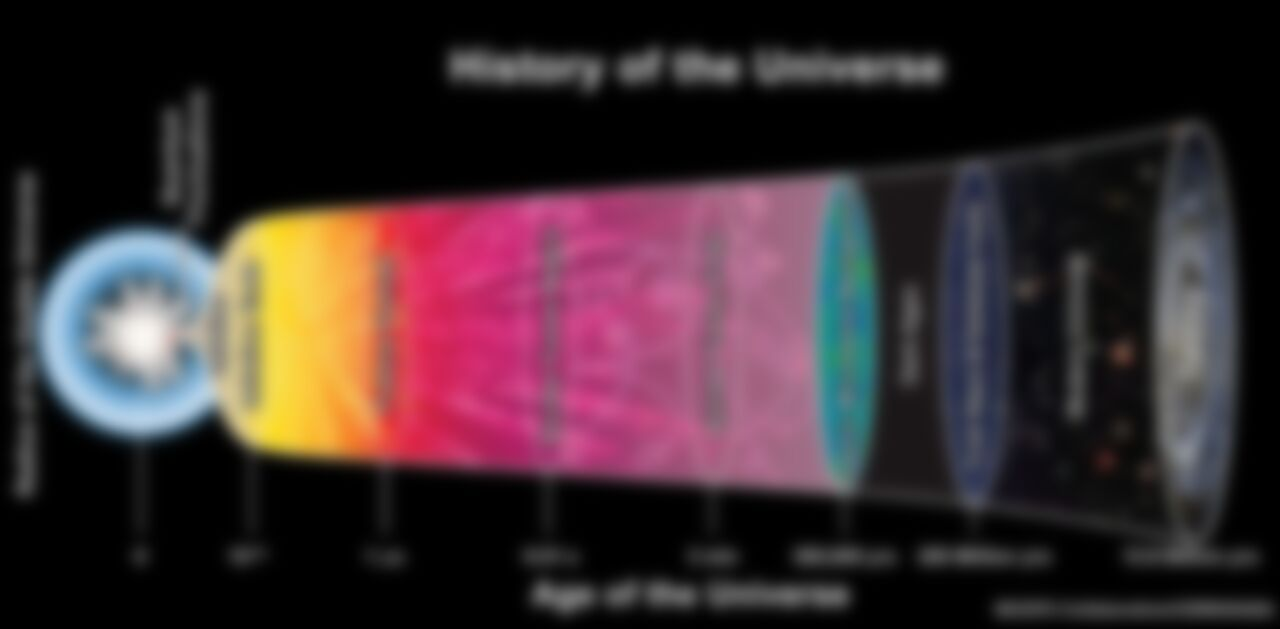
\includegraphics[height=5.5cm]{Plots/BigBangHistory_blur.jpg}}%
    \adjustbox{trim={0.82\width} {0} {0} {0},clip=true}{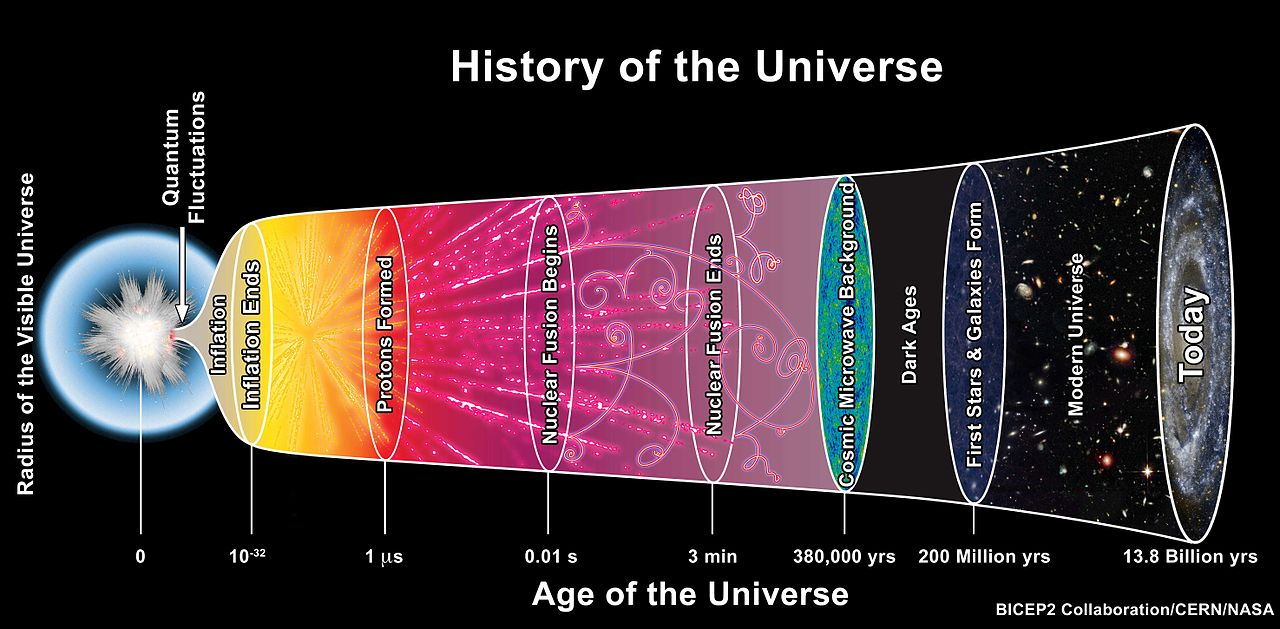
\includegraphics[height=5.5cm]{Plots/BigBangHistory.jpg}}
  \end{figure}
  \begin{center}
    \Large ... but today we only see matter!
  \end{center}
\end{frame}

\begin{frame}{Big Bang and matter-antimatter asymmetry}
  \begin{figure}
    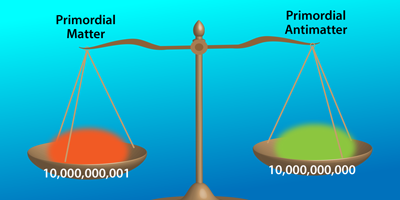
\includegraphics[width=0.8\textwidth,trim={0.9cm 0 0.9cm 0},clip=true]{Plots/PrimordialAntimatter.png}
    \caption*{\tiny APS/Alan Stonebraker}
  \end{figure}
  \vspace{-0.5cm}
  \begin{center}
    \Large The difference is very small...
  \end{center}
\end{frame}

\begin{frame}{Big Bang and matter-antimatter asymmetry}
  \begin{figure}
    
\includegraphics[width=0.45\textwidth]{Plots/MatterAntimatterBigAsymmetry.png}
    \caption*{\tiny Quantum Diaries: Why B physics? Why not A Physics?}
  \end{figure}
  \vspace{-0.5cm}
  \begin{center}
    \Large ... but the effects we observe today are obviously huge! How can we explain this?
  \end{center}
\end{frame}

\begin{frame}{$C\!P$ violation}
  \begin{columns}
    \begin{column}{0.4\textwidth}
      \begin{figure}
        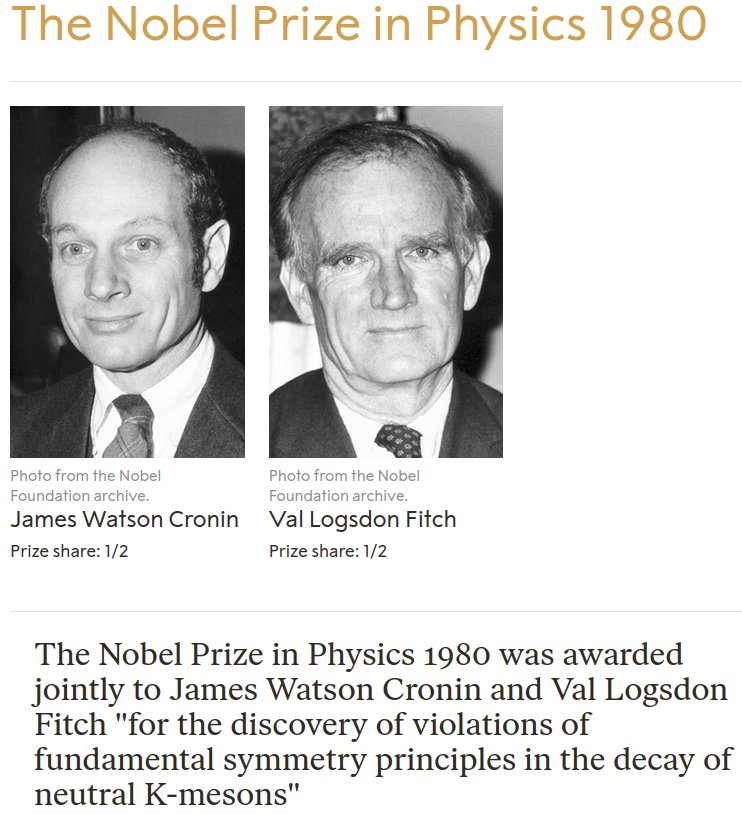
\includegraphics[width=1.0\textwidth]{Plots/NobelPrize1980.png}
      \end{figure}
    \end{column}
    \begin{column}{0.6\textwidth}
      \begin{itemize}
        \setlength\itemsep{1.0em}
        \item{$C\!P$ violation discovery in 1964}
        \item{Phys. Rev. Lett. \textbf{13}, 138}
        \item{Observed $K_L^0\to\pi^+\pi^-$}
        \item{Since, $C\!P$ violation has also been observed in the $B$, $B_s$ and $D$ systems}
      \end{itemize}
    \end{column}
  \end{columns}
  \vspace{0.5cm}
  \begin{center}
    \large Can Standard Model CPV explain the matter-antimatter asymmetry?\\Or, could it be physics beyond the SM?
  \end{center}
\end{frame}

\section{The CKM matrix and the Unitary Triangle}
\begin{frame}{The CKM matrix and the Unitary Triangle}
  \begin{center}
    {\huge The CKM matrix and the Unitary Triangle}
  \end{center}
\end{frame}

\begin{frame}{The CKM matrix and the Unitary Triangle}
  \begin{center}
    In SM, the charged current $W^\pm$ interactions couple (left-handed) up- and down-type quarks, given by
  \end{center}
  \begin{equation*}
    \frac{-g}{\sqrt{2}}
    \begin{bmatrix}
      \bar{u_L} & \bar{c_L} & \bar{t_L}
    \end{bmatrix}
    \gamma^\mu W_\mu V_{\rm CKM}
    \begin{bmatrix}
      d_L \\
      s_L \\
      b_L
    \end{bmatrix}
     + {\rm h.c.}
  \end{equation*}
  \begin{figure}[H]
    \centering
    \vspace{0.3cm}
    \begin{subfigure}{0.5\textwidth}
      \centering
      \begin{fmffile}{fgraph/fgraph_W1}
        \setlength{\unitlength}{0.4cm}
        \begin{fmfgraph*}(6,6)
          \fmfstraight
          \fmfleft{i1}
          \fmfright{o1,o2}
          \fmflabel{$t$}{i1}
          \fmflabel{$b$}{o1}
          \fmflabel{$W^+$}{o2}
          \fmf{fermion}{i1,v}
          \fmf{fermion}{v,o1}
          \fmf{boson}{v,o2}
        \end{fmfgraph*}
      \end{fmffile}
      \vspace{0.5cm}
      \caption{$t\to bW^+$}
    \end{subfigure}%
    \begin{subfigure}{0.5\textwidth}
      \centering
      \begin{fmffile}{fgraph/fgraph_W2}
        \setlength{\unitlength}{0.4cm}
        \begin{fmfgraph*}(6,6)
          \fmfstraight
          \fmfleft{i1}
          \fmfright{o1,o2}
          \fmflabel{$b$}{i1}
          \fmflabel{$c$}{o1}
          \fmflabel{$W^-$}{o2}
          \fmf{fermion}{i1,v}
          \fmf{fermion}{v,o1}
          \fmf{boson}{v,o2}
        \end{fmfgraph*}
      \end{fmffile}
      \vspace{0.5cm}
      \caption{$b\to cW^-$}
    \end{subfigure}
  \end{figure}
\end{frame}

\begin{frame}{The CKM matrix and the Unitary Triangle}
  \begin{center}
    The Cabbibo-Kobayashi-Maskawa matrix $V_{\rm CKM}$,
  \end{center}
  \begin{equation*}
    \begin{bmatrix}
      V_{ud} & V_{us} & V_{ub} \\
      V_{cd} & V_{cs} & V_{cb} \\
      V_{td} & V_{ts} & V_{tb}
    \end{bmatrix}
  \end{equation*}
  \begin{center}
    must be a unitary matrix: $V^\dagger_{\rm CKM}V_{\rm CKM} = I\implies$
  \end{center}
  \vspace{0.5cm}
  \begin{equation*}
    V^{\phantom{*}}_{ud}V^*_{ub} + V^{\phantom{*}}_{cd}V^*_{cb} + V^{\phantom{*}}_{td}V^*_{tb} = 0
  \end{equation*}
  \begin{center}
    Represent this constraint as a triangle in the complex plane:\\Unitary Triangle
  \end{center}
\end{frame}

\begin{frame}{The CKM matrix and the Unitary Triangle}
  \begin{itemize}
    \setlength\itemsep{0.3em}
    \item{CPV in SM is described by the Unitary Triangle, with angles $\alpha$, $\beta$, $\gamma$}
    \item{The angle $\gamma = \text{arg}\Big(-\frac{V^{\phantom{*}}_{ud}V^*_{ub}}{V^{\phantom{*}}_{cd}V^*_{cb}}\Big)$ is very important:}
    \begin{enumerate}
    \setlength\itemsep{0.2em}
      \item{Negligible theoretical uncertainties: Ideal SM benchmark}
      \item{Accessible at tree level: Indirectly probe New Physics that enter loops}
      \item{Compare with $\alpha$, $\beta$ measurements: Is the Unitary Triangle a triangle?}
    \end{enumerate}
  \end{itemize}
  \vspace{-0.2cm}
  \begin{figure}
    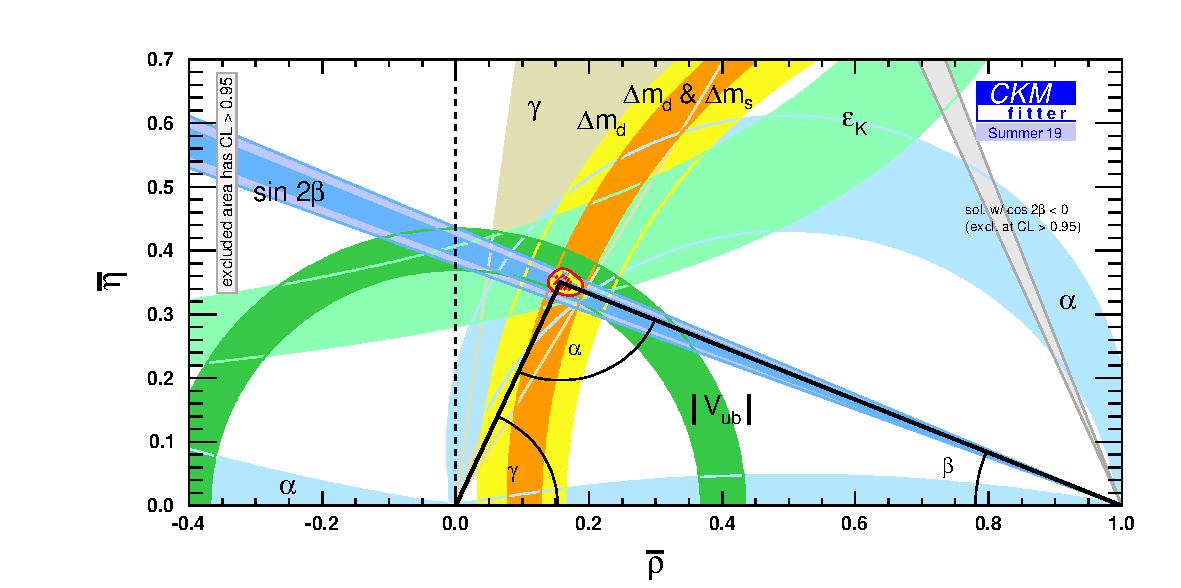
\includegraphics[width = 0.70\textwidth]{Plots/ckmfitter2.pdf}
    \vspace{-0.3cm}
    \caption*{\tiny CKMfitter Group (J. Charles et al.), Eur. Phys. J. C41, 1-131 (2005)}
  \end{figure}
\end{frame}

\section{How to measure \texorpdfstring{$\gamma$}{gamma}?}
\begin{frame}{How to measure $\gamma$?}
  \begin{center}
    {\huge How to measure $\gamma$?}
  \end{center}
\end{frame}

\begin{frame}{Sensitivity through interference}
  \begin{center}
    \Large Measure $\gamma$ through interference effects in $B^\pm\to DK^\pm$
  \end{center}
  \begin{figure}[H]
    \centering
    \begin{subfigure}{0.5\textwidth}
      \centering
      \begin{fmffile}{fgraph/fgraph_BtoDK1}
        \setlength{\unitlength}{0.4cm}
        \begin{fmfgraph*}(6,6)
          \fmfstraight
          \fmfleft{i1,B,i2,t1,t2,t3,t9,t10}
          \fmfright{o1,D,o2,t4,t5,o3,K,o4}
          \fmflabel{$\bar{u}$}{i1}
          \fmflabel{$b$}{i2}
          \fmfv{l.d=20,l.a=180,l={$B^-$\mylbrace{30}{-8}}}{B}
          \fmflabel{$\bar{u}$}{o1}
          \fmflabel{$c$}{o2}
          \fmflabel{$\bar{u}$}{o3}
          \fmflabel{$s$}{o4}
          \fmfv{l.d=15,l.a=0,l={\myrbrace{30}{-12}}$D^0$}{D}
          \fmfv{l.d=15,l.a=0,l={\myrbrace{30}{11}}$K^-$}{K}
          \fmf{fermion}{o1,i1}
          \fmf{fermion,tension=1.5}{i2,v1}
          \fmf{fermion}{v1,o2}
          \fmf{phantom,tension=1.5}{t9,v2}
          \fmf{boson,label=$W$,label.side=left,tension=0}{v1,v2}
          \fmf{fermion}{v2,o4}
          \fmf{fermion}{o3,v2}
        \end{fmfgraph*}
      \end{fmffile}
      \vspace{0.5cm}
      \caption*{Favoured $B^-\to D^0K^-$}
    \end{subfigure}%
    \begin{subfigure}{0.5\textwidth}
      \centering
      \begin{fmffile}{fgraph/fgraph_BtoDK2}
        \setlength{\unitlength}{0.4cm}
        \begin{fmfgraph*}(6,6)
          \fmfstraight
          \fmfleft{i1,t1,t2,B,t9,t10,i2}
          \fmfright{o1,K,o2,t4,t5,o3,D,o4}
          \fmflabel{$\bar{u}$}{i1}
          \fmflabel{$b$}{i2}
          \fmfv{l.d=20,l.a=180,l={$B^-$\mylbrace{100}{-8}}}{B}
          \fmflabel{$\bar{u}$}{o1}
          \fmflabel{$s$}{o2}
          \fmflabel{$\bar{c}$}{o3}
          \fmflabel{$u$}{o4}
          \fmfv{l.d=15,l.a=0,l={\myrbrace{30}{13}}$\bar{D^0}$}{D}
          \fmfv{l.d=15,l.a=0,l={\myrbrace{30}{-13}}$K^-$}{K}
          \fmf{fermion}{o1,i1}
          \fmf{fermion,tension=1.5}{i2,v1}
          \fmf{fermion}{v1,o4}
          \fmf{phantom,tension=1.5}{t2,v2}
          \fmf{boson,label=$W$,label.side=left,tension=0}{v1,v2}
          \fmf{fermion}{v2,o2}
          \fmf{fermion}{o3,v2}
        \end{fmfgraph*}
      \end{fmffile}
      \vspace{0.5cm}
      \caption*{Suppressed $B^-\to\bar{D^0}K^-$}
    \end{subfigure}
  \end{figure}
  \vspace{-0.3cm}
  \begin{itemize}
    \item{Superposition of $D^0$ and $\bar{D^0}$}
    \item{$b\to u\bar{c}s$ and $b\to c\bar{u}s$ interference $\to$ Sensitivity to $\gamma$}
  \end{itemize}
  \vspace{-0.3cm}
  \begin{center}
    $\mathcal{A}(B^-)\propto\mathcal{A}(D^0) + r_Be^{i(\delta_B - \gamma)}\mathcal{A}(\bar{D^0})$ \\
    $\mathcal{A}(B^+)\propto\mathcal{A}(\bar{D^0}) + r_Be^{i(\delta_B + \gamma)}\mathcal{A}(D^0)$ \\
  \end{center}
  \vspace{-0.3cm}
  \begin{itemize}
    \item{The magnitude of interference effects governed by $r_B\approx0.1$}
  \end{itemize}
\end{frame}

\begin{frame}[fragile]{$D$ decays to a $C\!P$ eigenstate}
  \begin{center}
    A well known strategy is to consider $D$ decays to a $C\!P$ eigenstate\\~\\
    For $C\!P$ eigenstates, $\mathcal{A}(D^0) = \mathcal{A}(\bar{D^0})$
  \end{center}
  \begin{equation*}
    \begin{tikzcd}[column sep=huge]
      & D^0K^- \arrow[dr, bend left = 25, "\mathcal{A}_{D^0}"] & \\
      B^- \arrow[ur, bend left, "\mathcal{A}_B"] \arrow[dr, bend right, "\mathcal{A}_B r_B e^{i(\delta_B - \gamma)}"'] & [5cm] & DK^- \\
      & \bar{D^0}K^- \arrow[ur, bend right = 25, "\mathcal{A}_{D^0}"'] & \\
    \end{tikzcd}
  \end{equation*}
  \begin{equation*}
    \lvert\mathcal{A}(B^-)\lvert^2\propto\lvert\mathcal{A}(D^0)\lvert^2\Big(1 + r_B^2 + 2r_B\cos(\delta_B - \gamma)\Big)
  \end{equation*}
\end{frame}

\begin{frame}{$D$ decays to a $C\!P$ eigenstate}
  \begin{figure}
    \centering
    \begin{subfigure}{0.45\textwidth}
      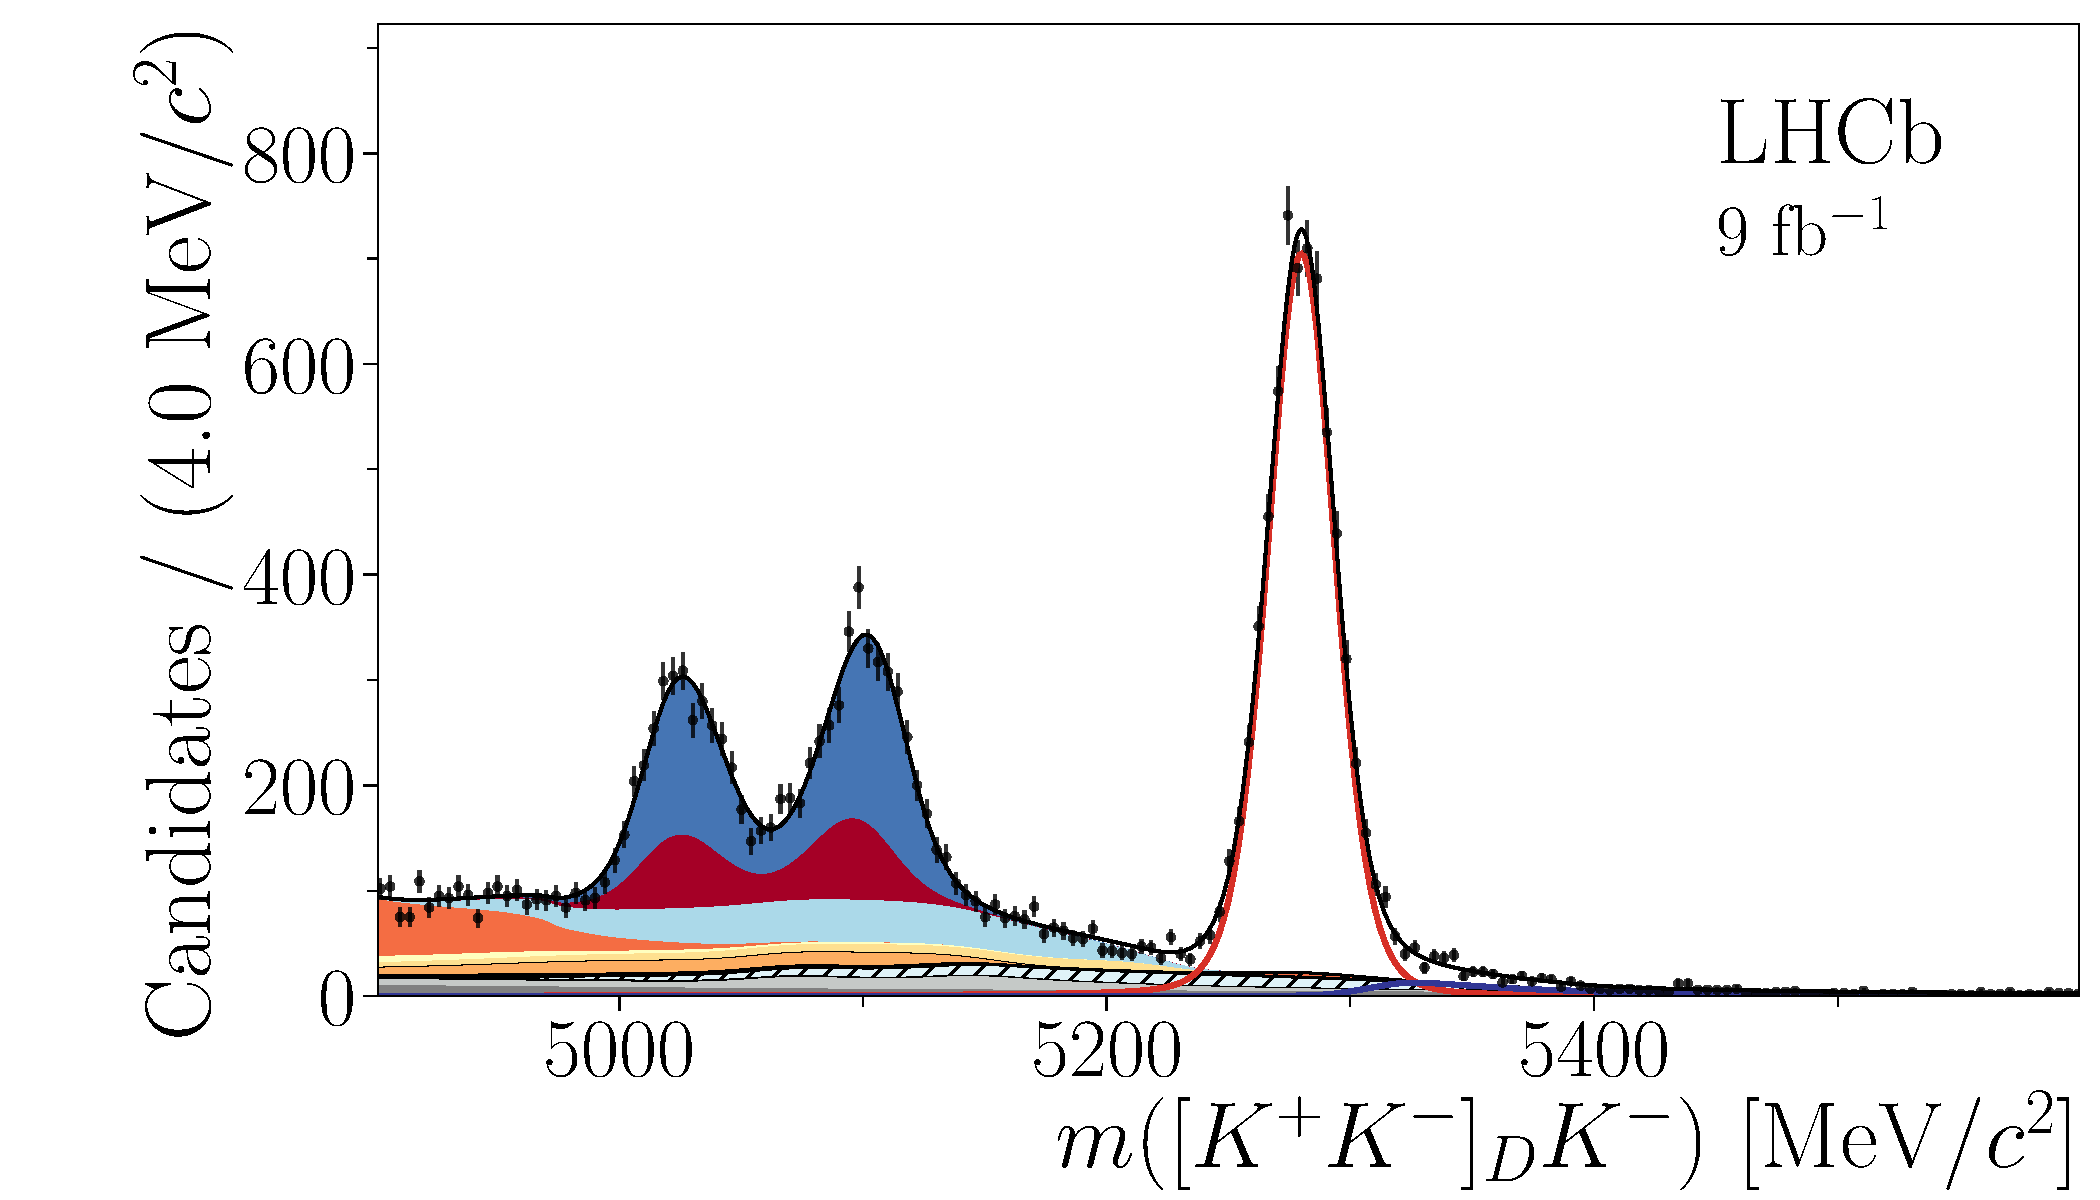
\includegraphics[width = 1.0\textwidth]{Plots/B2DK_D2KK_Minus.pdf}
    \end{subfigure}%
    \begin{subfigure}{0.45\textwidth}
      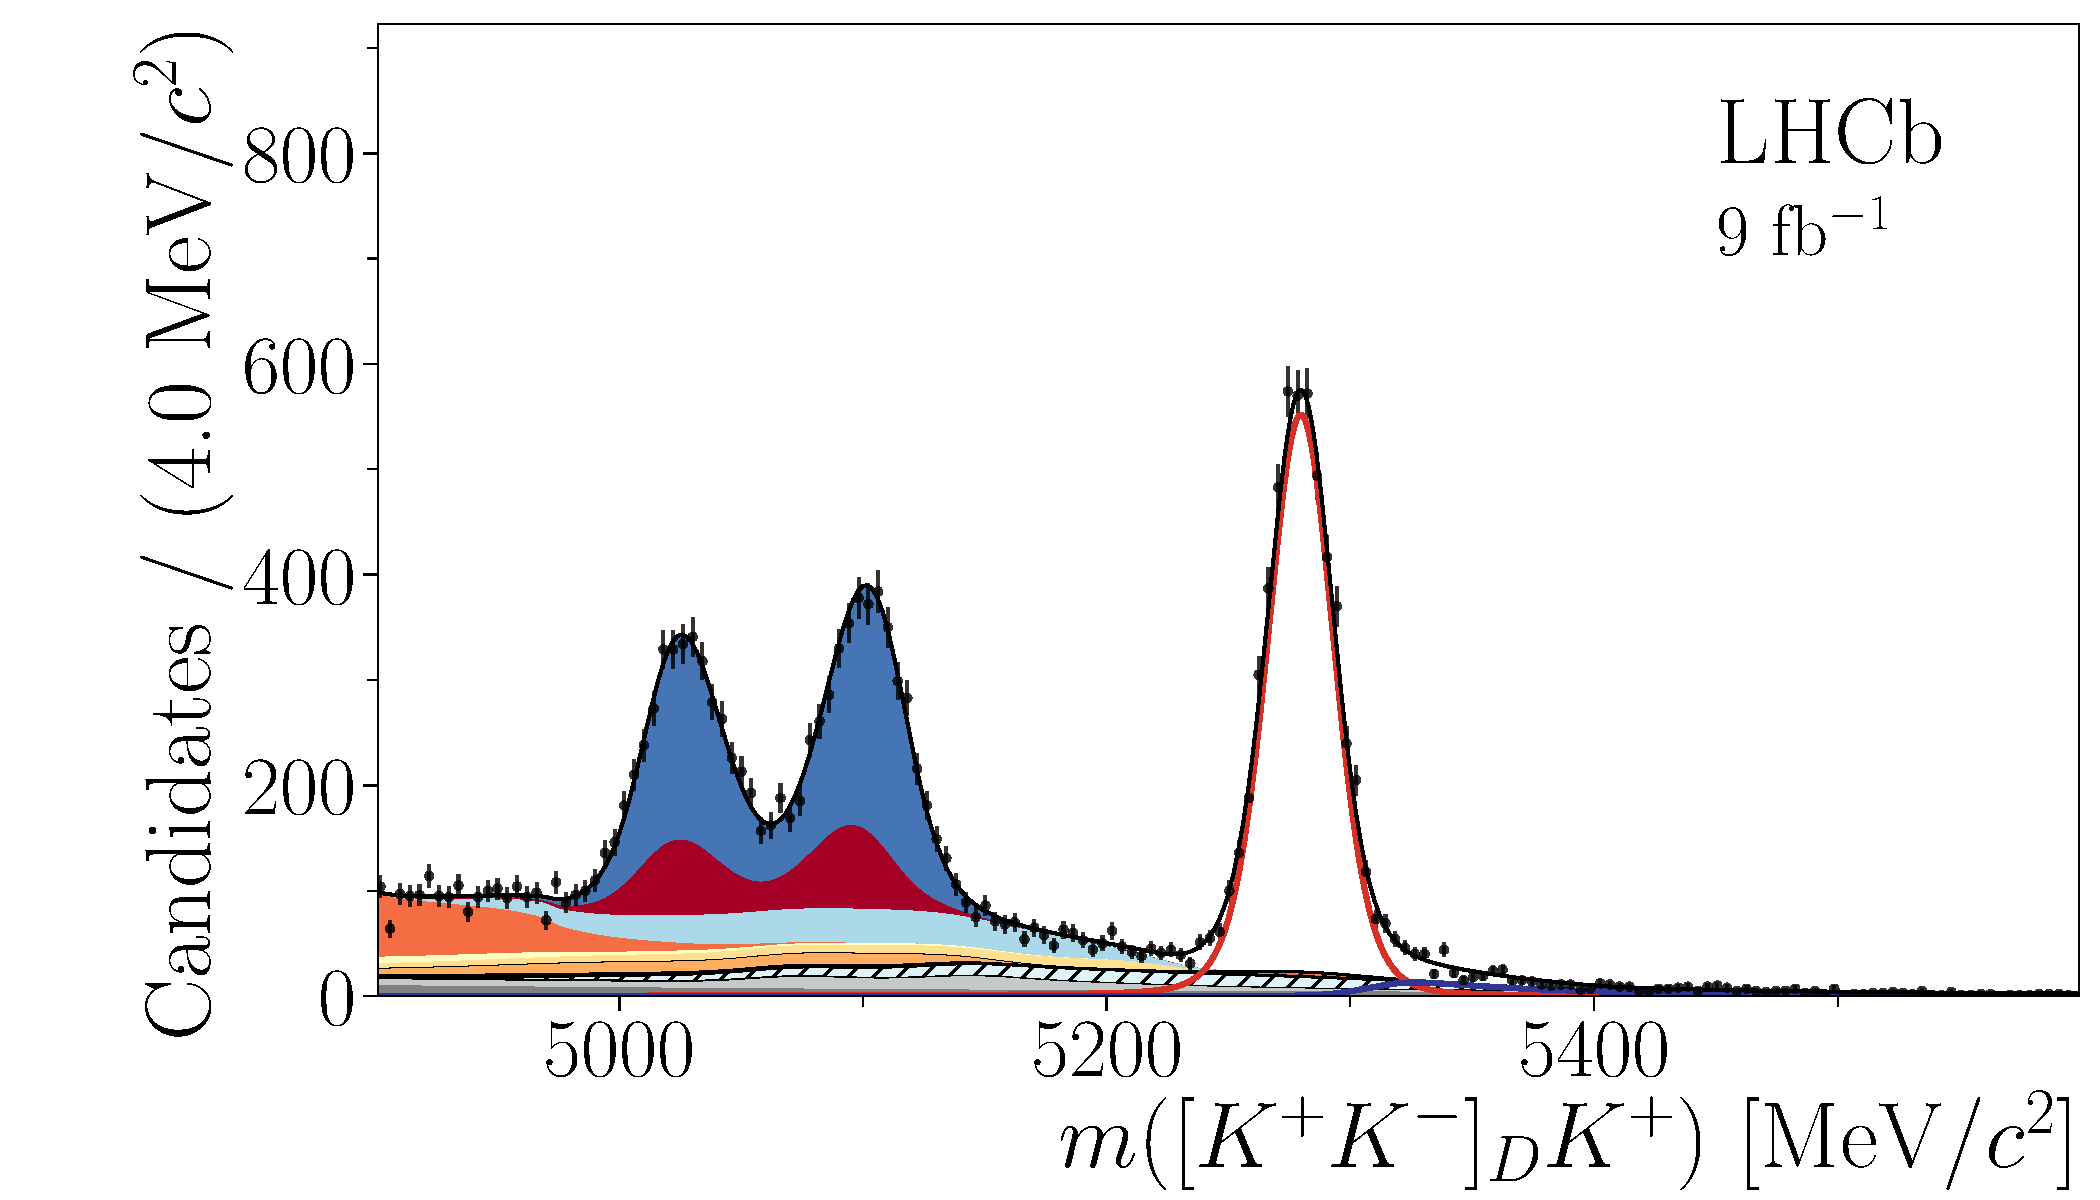
\includegraphics[width = 1.0\textwidth]{Plots/B2DK_D2KK_Plus.pdf}
    \end{subfigure}
    \begin{subfigure}{0.45\textwidth}
      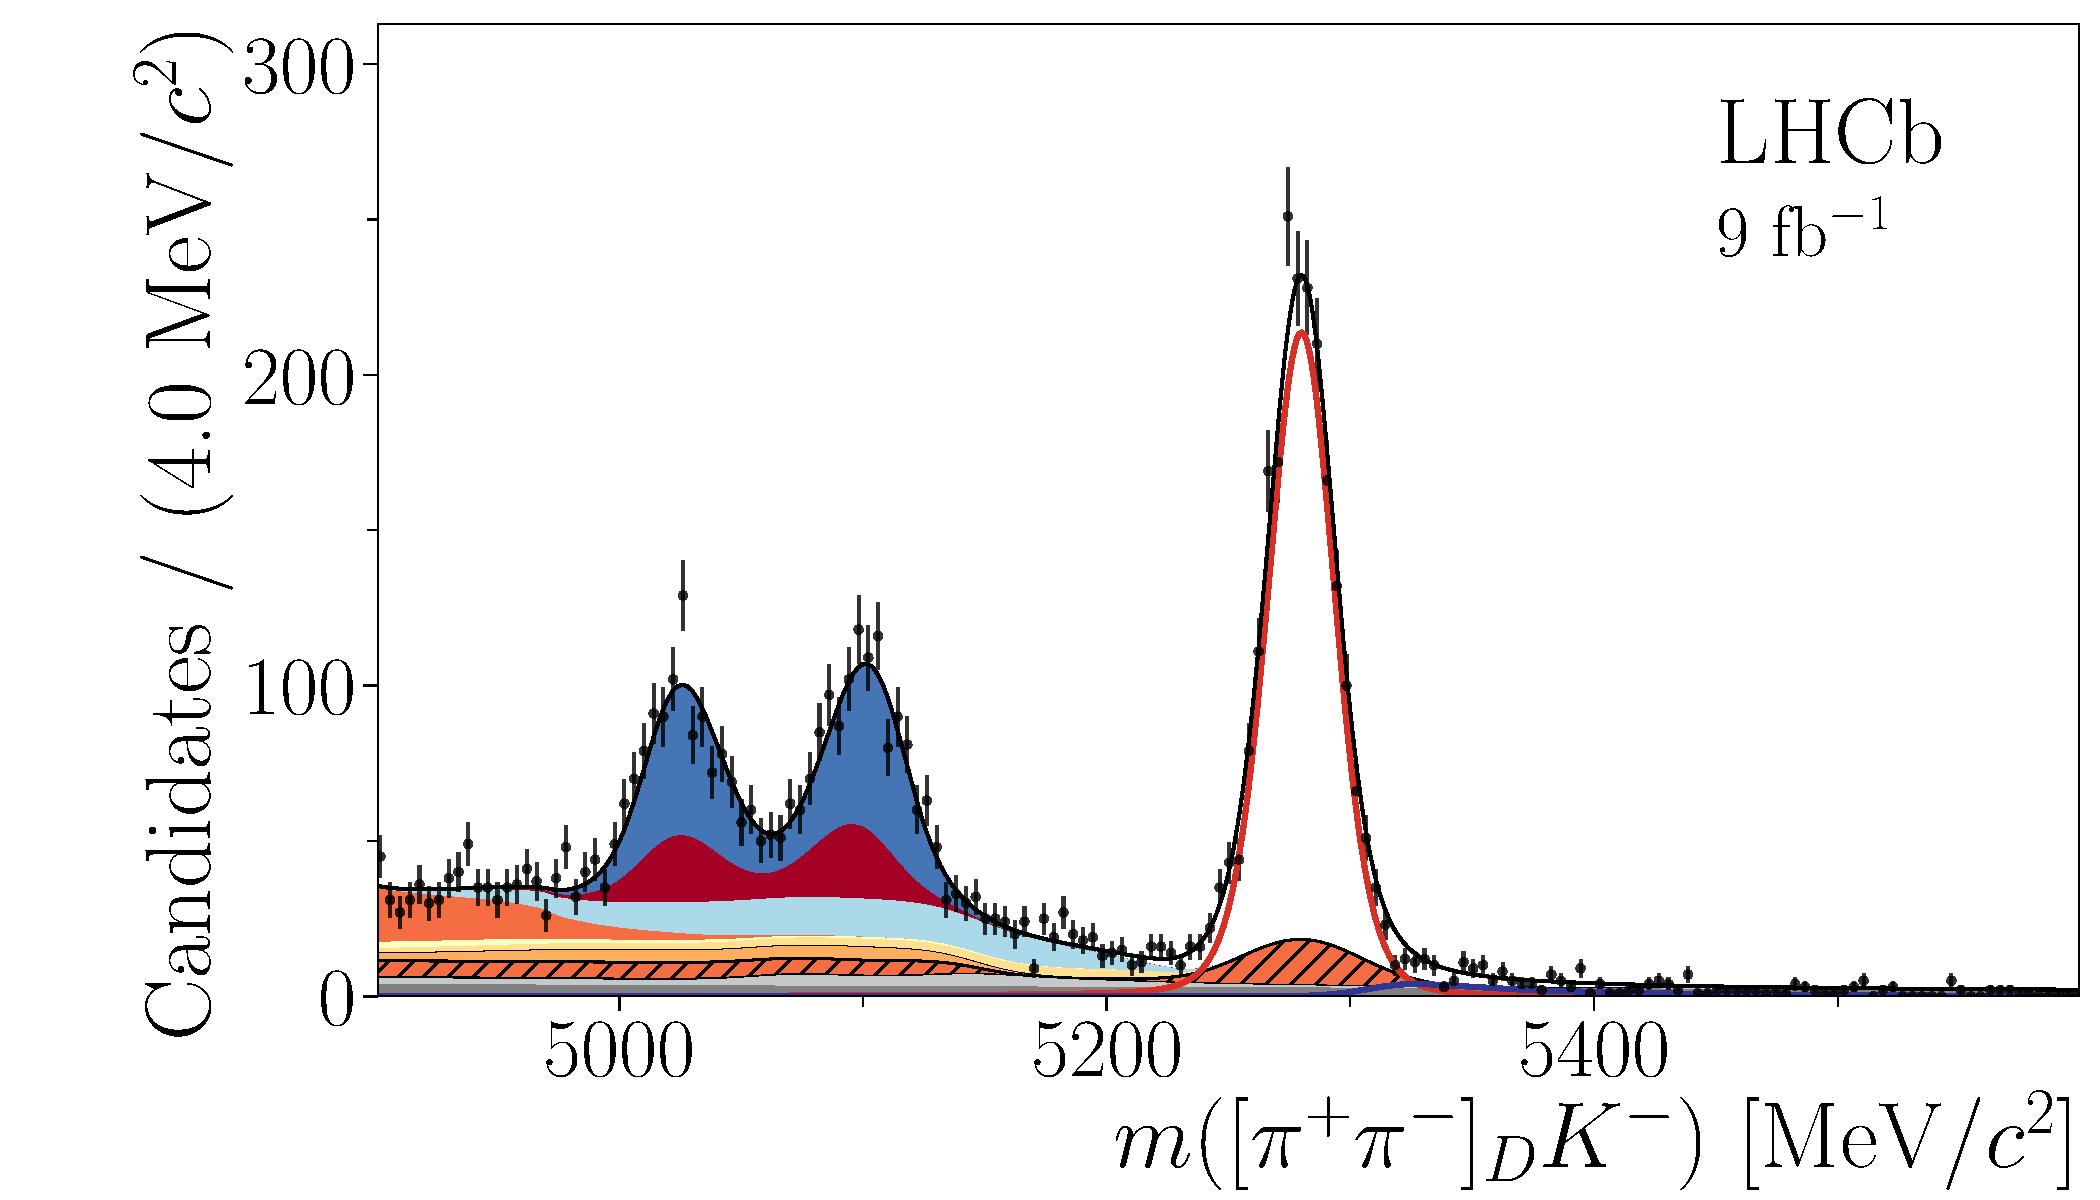
\includegraphics[width = 1.0\textwidth]{Plots/B2DK_D2pipi_Minus.pdf}
    \end{subfigure}%
    \begin{subfigure}{0.45\textwidth}
      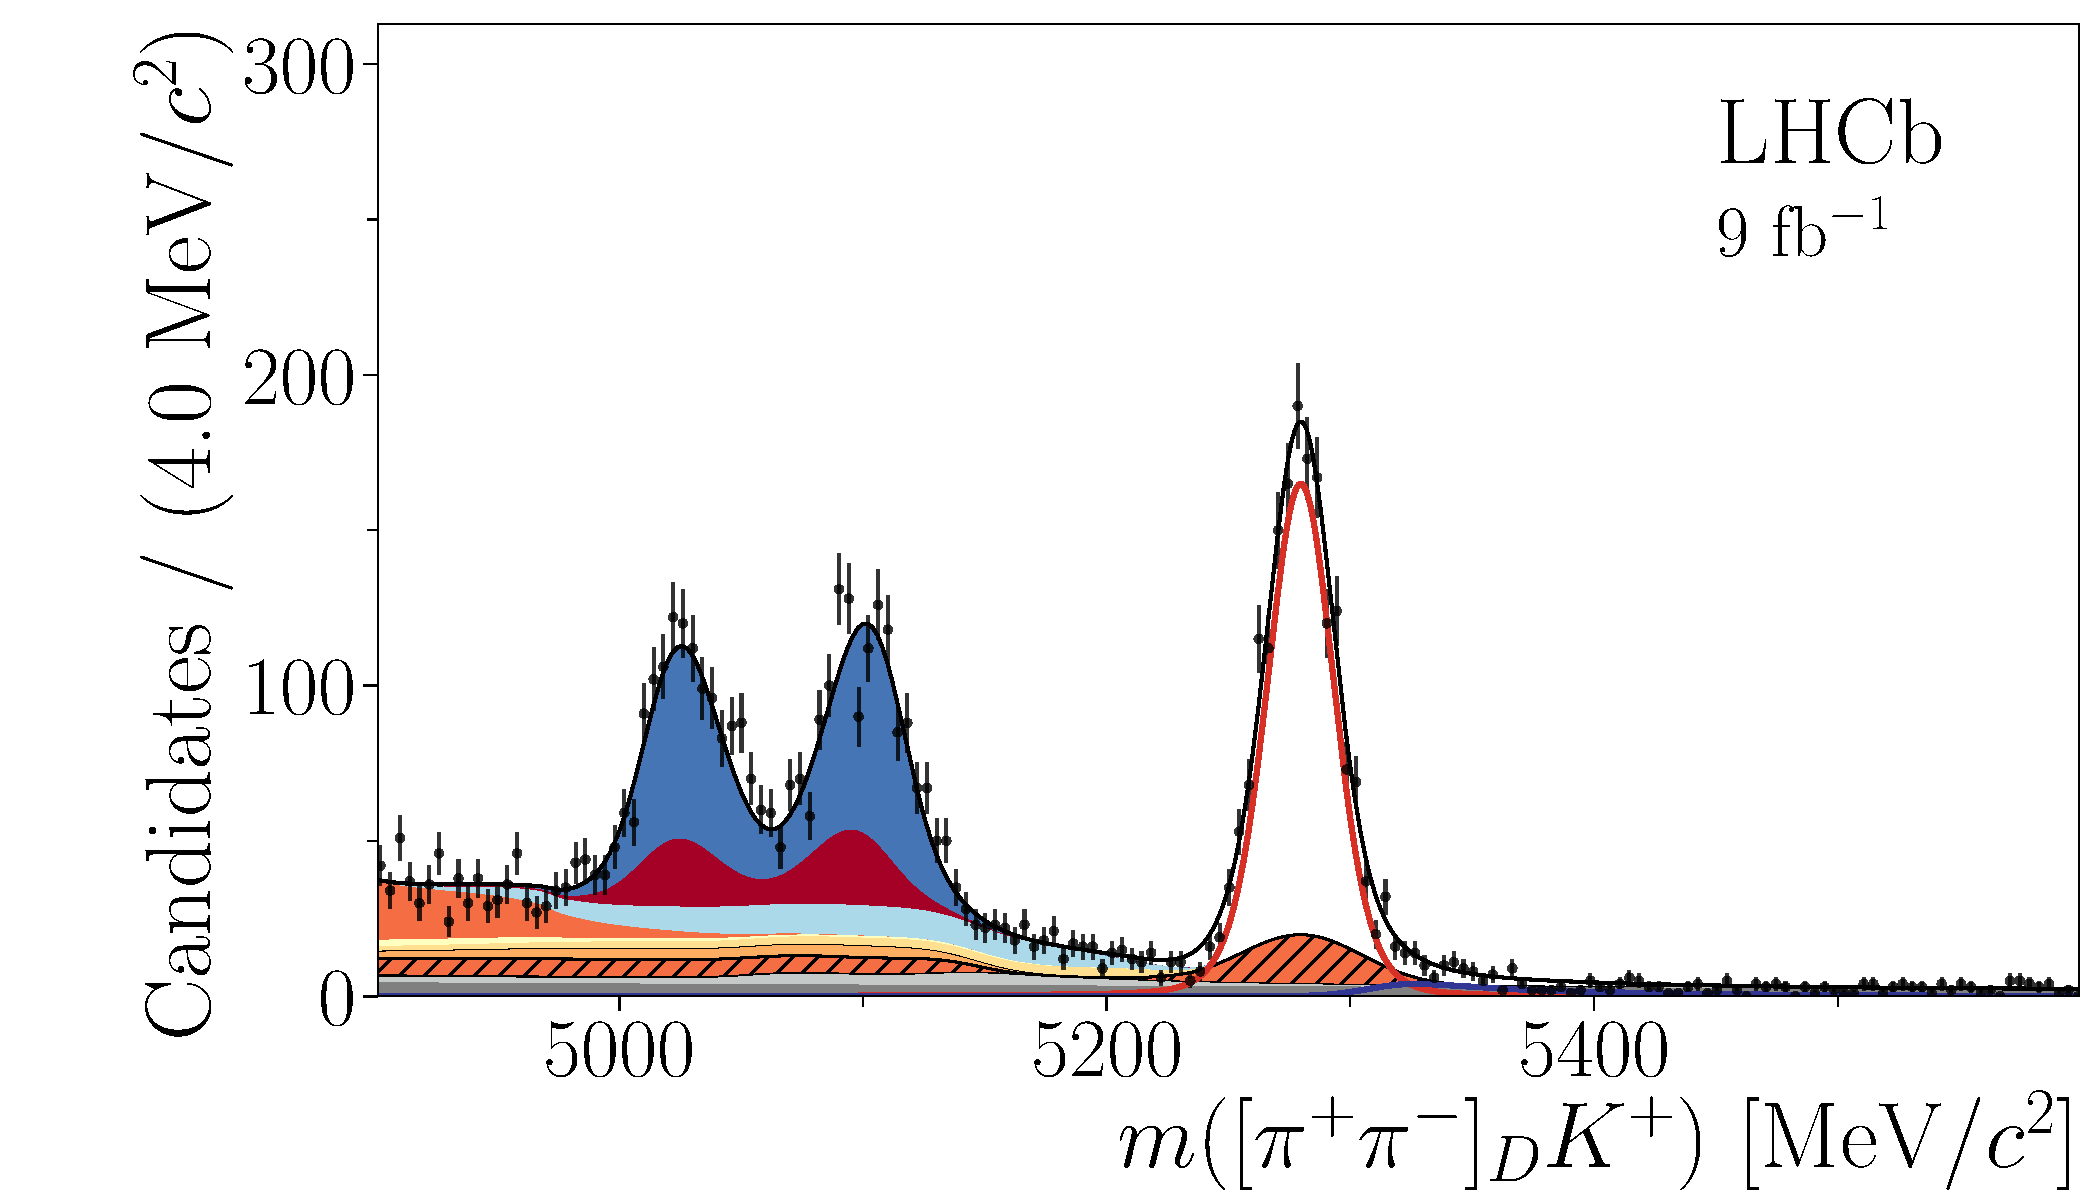
\includegraphics[width = 1.0\textwidth]{Plots/B2DK_D2pipi_Plus.pdf}
    \end{subfigure}
    \caption*{\tiny JHEP \textbf{04} (2021) 081}
  \end{figure}
  \vspace{-0.5cm}
  \begin{center}
    \Large In $B^\pm\to[h^+h^-]_DK^\pm$, we see large CPV effects!
  \end{center}
\end{frame}

\begin{frame}[fragile]{Doubly Suppressed Cabbibo $D$ decays}
  \begin{center}
    Can we enhance the interference effects?\\~\\
    Yes! Use a Doubly Suppressed Cabbibo decay: $\mathcal{A}(D^0) = r_De^{i\delta_D}\mathcal{A}(\bar{D^0})$
  \end{center}
  \begin{equation*}
    \begin{tikzcd}[column sep=huge]
      & D^0K^- \arrow[dr, bend left = 25, "r_De^{i\delta_D}\mathcal{A}_{\bar{D^0}}"] & \\
      B^- \arrow[ur, bend left, "\mathcal{A}_B"] \arrow[dr, bend right, "\mathcal{A}_B r_B e^{i(\delta_B - \gamma)}"'] & [5cm] & DK^- \\
      & \bar{D^0}K^- \arrow[ur, bend right = 25, "\mathcal{A}_{\bar{D^0}}"'] & \\
    \end{tikzcd}
  \end{equation*}
  \begin{equation*}
    \lvert\mathcal{A}(B^-)\lvert^2\propto\lvert\mathcal{A}(D^0)\lvert^2\Big(r_D^2 + r_B^2 + 2r_Br_D\cos(\delta_B - \gamma + \delta_D)\Big)
  \end{equation*}
\end{frame}

\begin{frame}{Doubly Suppressed Cabbibo $D$ decays}
  \begin{figure}
    \centering
    \begin{subfigure}{0.5\textwidth}
      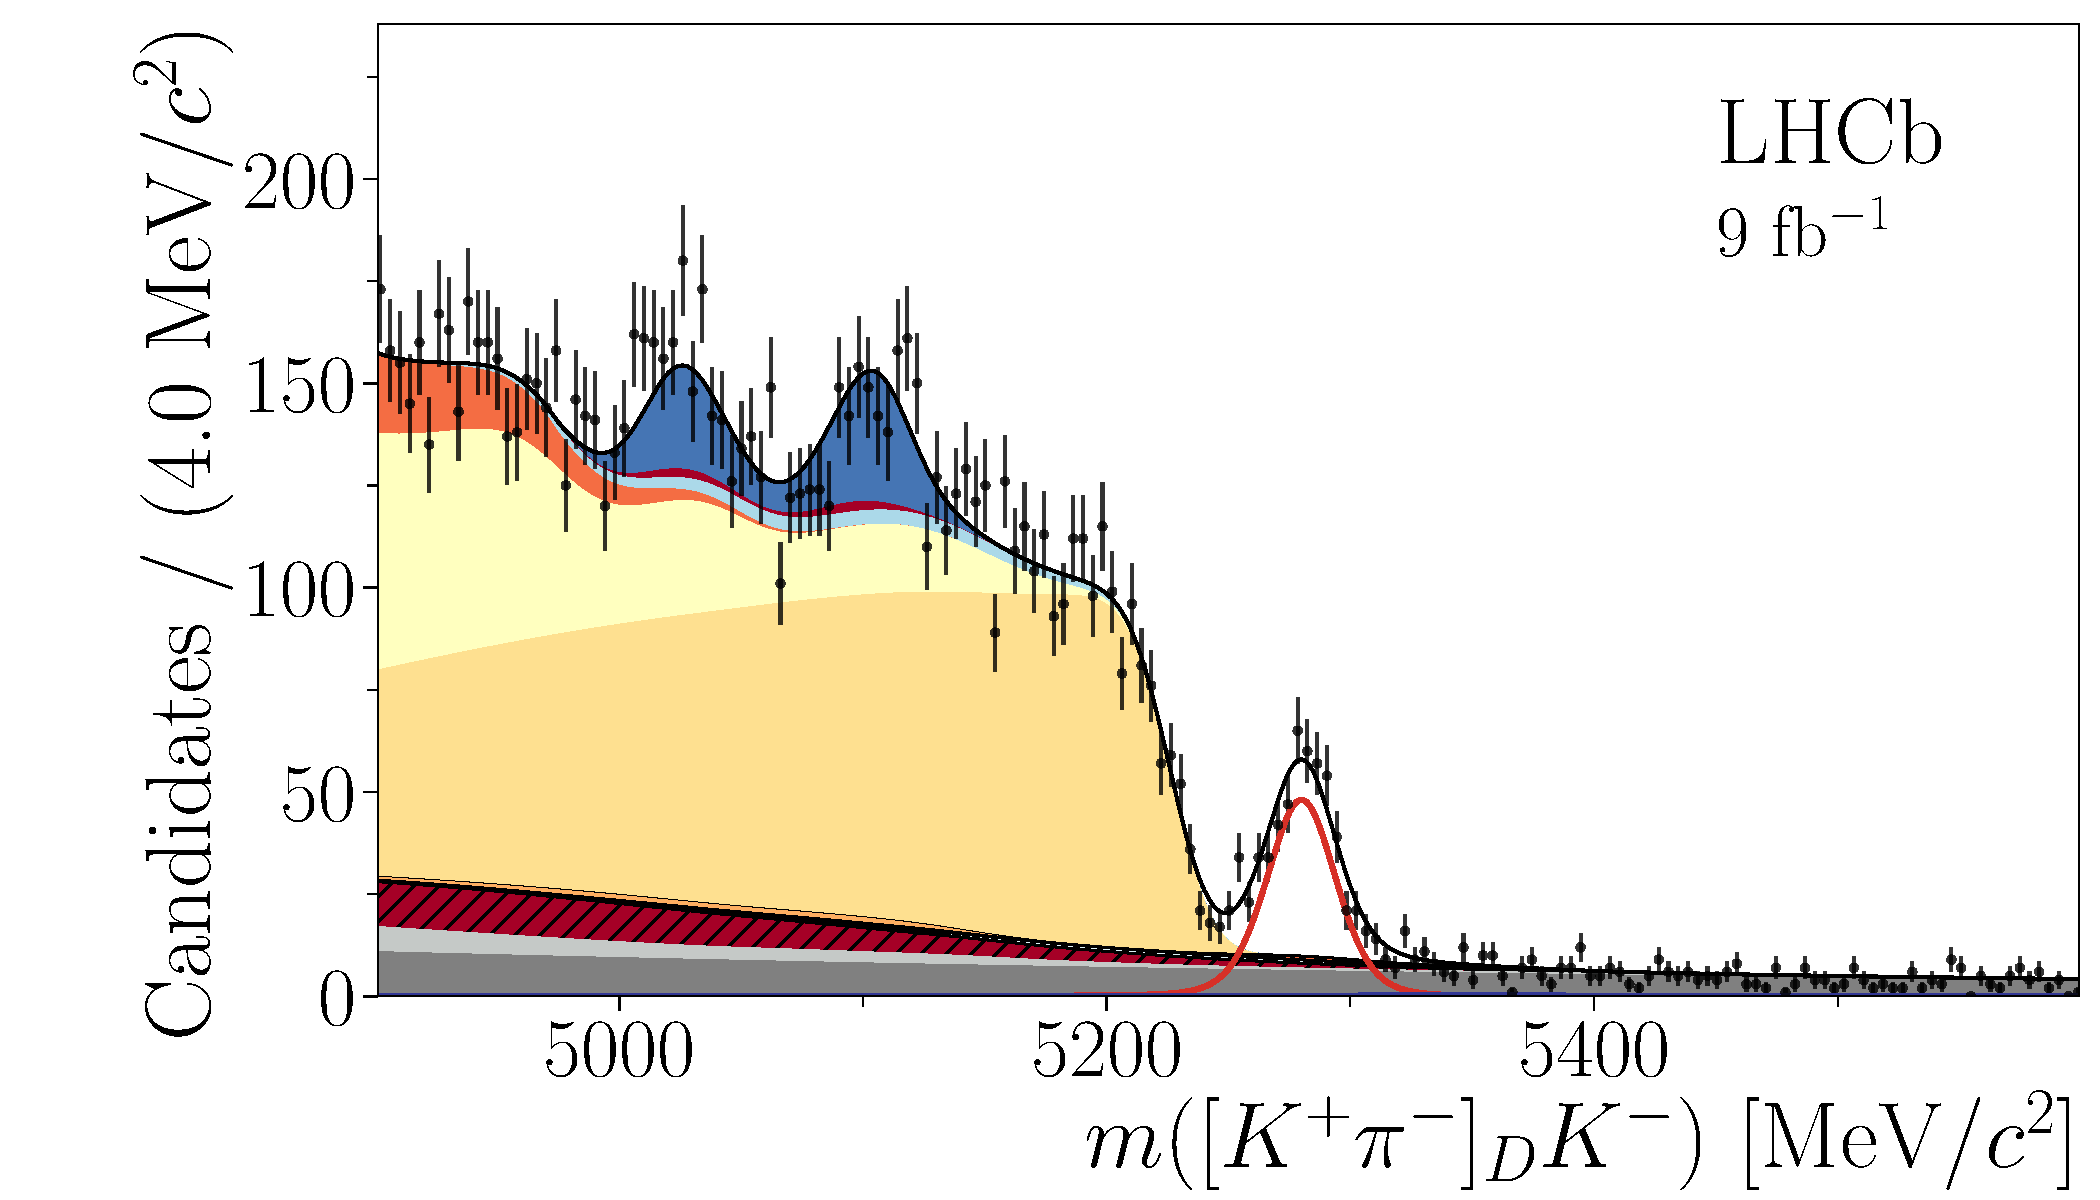
\includegraphics[width = 1.0\textwidth]{Plots/B2DK_D2Kpi_Minus.pdf}
    \end{subfigure}%
    \begin{subfigure}{0.5\textwidth}
      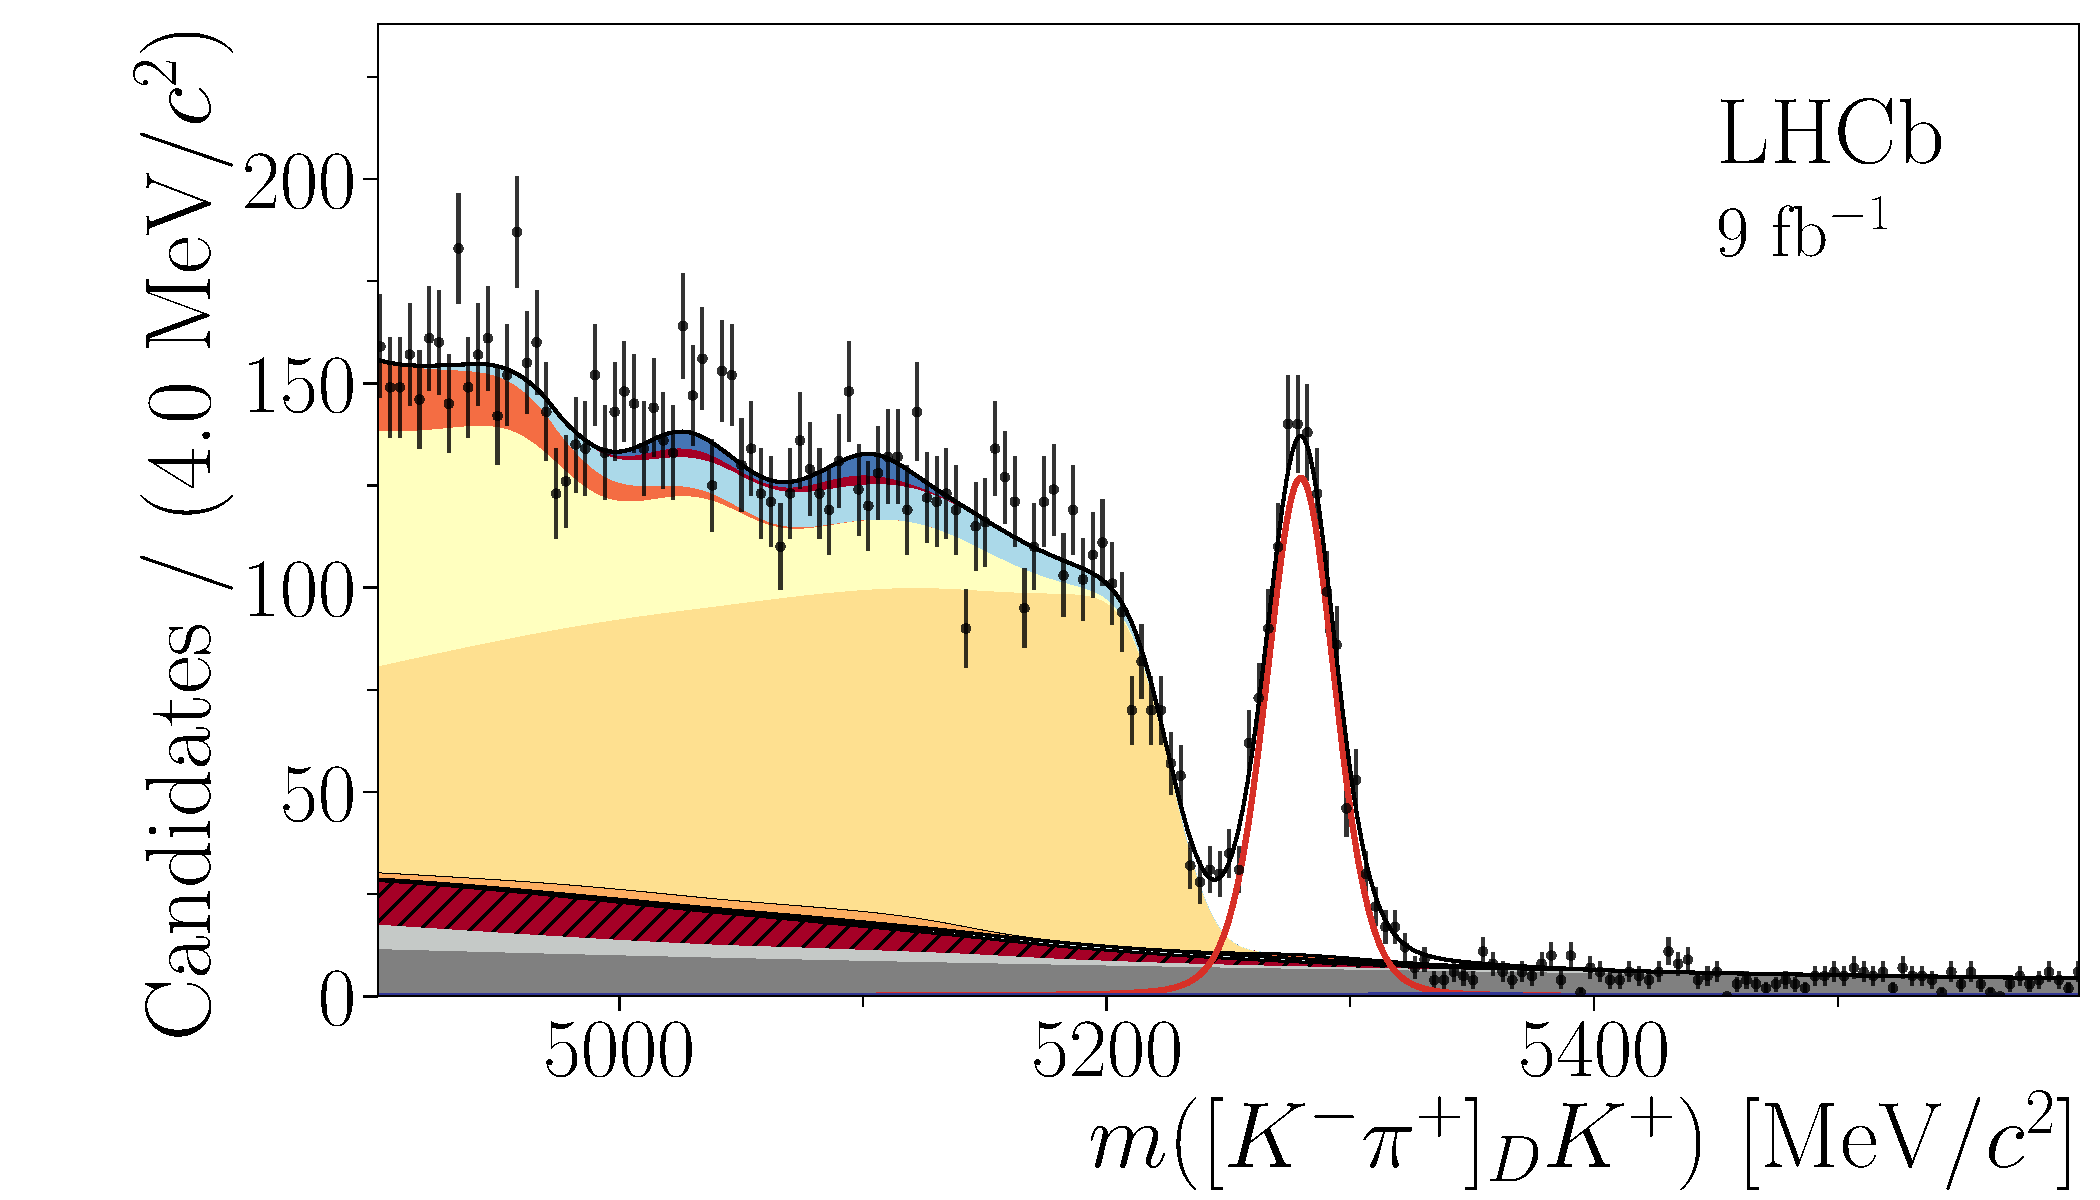
\includegraphics[width = 1.0\textwidth]{Plots/B2DK_D2Kpi_Plus.pdf}
    \end{subfigure}
    \caption*{\tiny JHEP \textbf{04} (2021) 081}
  \end{figure}
  \vspace{-0.5cm}
  \begin{center}
    \Large $B^\pm\to[K^\mp\pi^\pm]_DK^\pm$ has lower statistics, but a spectacular asymmetry!\\~\\
    \large Additionally, the partially reconstructed background has an equal but opposite asymmetry
  \end{center}
\end{frame}

\section{The \texorpdfstring{$B^\pm\to[K^+K^-\pi^+\pi^-]_DK^\pm$}{B2DK_D2KKpipi} decay mode}
\begin{frame}{The $B^\pm\to[K^+K^-\pi^+\pi^-]_DK^\pm$ decay mode}
  \begin{center}
    {\huge The $B^\pm\to[K^+K^-\pi^+\pi^-]_DK^\pm$ decay mode}
  \end{center}
\end{frame}

\begin{frame}{The $B^\pm\to[K^+K^-\pi^+\pi^-]_DK^\pm$ decay mode}
  \begin{center}
    \Large The mode $B^\pm\to[K^+K^-\pi^+\pi^-]_DK^\pm$ has been proposed as a powerful channel for a measurement of $\gamma$
  \end{center}
  \begin{itemize}
    \setlength\itemsep{1.2em}
    \item{First proposed by J. Rademacker and G. Wilkinson}
    \begin{itemize}
      \item{Phys. Lett. \textbf{B647} (2007) 400}
      \item{Amplitude model by FOCUS}
      \item{Expected $\gamma$ precision from amplitude fit with $1000$ candidates: $14^\circ$}
    \end{itemize}
    \item{State of the art amplitude analysis by LHCb:}
    \begin{itemize}
      \item{JHEP \textbf{02} (2019) 126}
      \item{Exploits the huge dataset of charm decays at LHCb}
    \end{itemize}
    \item{$D\to K^+K^-\pi^+\pi^-$ has the best of both worlds:}
    \begin{itemize}
      \item{Singly Suppressed Cabbibo decay: Larger branching fraction}
      \item{Large interference effects in some regions of phase space}
    \end{itemize}
  \end{itemize}
\end{frame}

\section{Binned \texorpdfstring{$\gamma$}{gamma} analysis of the \texorpdfstring{$D\to K^+K^-\pi^+\pi^-$}{D->KKpipi} mode}
\begin{frame}{The $D\to K^+K^-\pi^+\pi^-$ decay}
  \begin{center}
    {\huge Binned $\gamma$ analysis of the $D\to K^+K^-\pi^+\pi^-$ mode}
  \end{center}
\end{frame}

\begin{frame}{Binned measurement of $\gamma$}
  \begin{itemize}
    \setlength\itemsep{0.5em}
    \item{Final measurement will be \underline{model-independent}}
    \begin{itemize}
      \item{Poor binning reduces statistical sensitivity $\to$ No bias!}
    \end{itemize}
    \item{Need strong phases of $D$ decay $\to$ Measure at BESIII}
    \item{LHCb-PAPER-2020-019: $B^\pm\to Dh^\pm$, $D\to K_S^0 h^+h^-$}
    \begin{itemize}
      \item{Single most precise measurement: $\gamma = (68.7^{+5.2}_{-5.1})^\circ$}
    \end{itemize}
  \end{itemize}
  \begin{figure}
    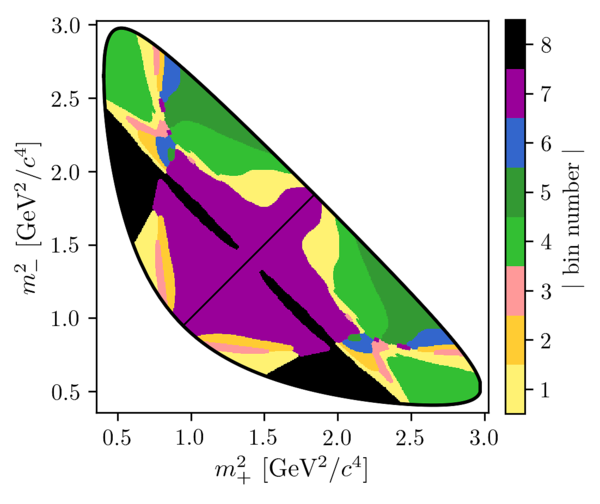
\includegraphics[height = 4cm]{Plots/KsPiPi_optimal.png}
    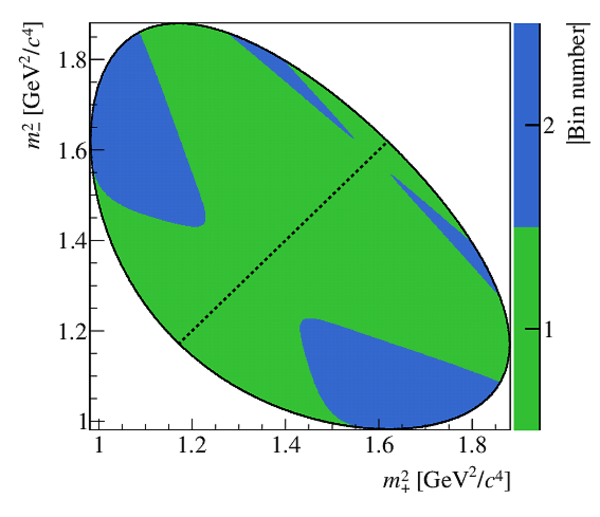
\includegraphics[height = 4cm]{Plots/KsKK_binning.png}
  \end{figure}
\end{frame}

\begin{frame}{The BPGGSZ method}
  \begin{itemize}
    \item{$B^\pm\to Dh^\pm$ amplitude:}
  \end{itemize}
  \begin{center}
    $\mathcal{A}(B^-) = \mathcal{A}(D^0) + r_Be^{i(\delta_B - \gamma)}\mathcal{A}(\bar{D^0})$ \\
    $\mathcal{A}(B^+) = \mathcal{A}(\bar{D^0}) + r_Be^{i(\delta_B + \gamma)}\mathcal{A}(D^0)$ \\
  \end{center}
  \begin{itemize}
    \item{$\mathcal{A}(D^0)$ and $\mathcal{A}(\bar{D^0})$ depend on $D$ phase space}
    \item{Strong-phase difference of $D^0$ and $\bar{D^0}$ decays inaccessible at LHCb}
    \item{Model-independent measurement: Integrate over bins of phase space}
  \end{itemize}
  \begin{block}{Event yield in bin $i$}
    $N^-_i = h_{B^-}\Big(F_i + \big(x_-^2 + y_-^2\big)\bar{F_i} + 2\sqrt{F_i\bar{F_i}}\big(x_-c_i + y_-s_i\big)\Big)$
    $N^+_{-i} = h_{B^+}\Big(F_i + \big(x_+^2 + y_+^2\big)\bar{F_i} + 2\sqrt{F_i\bar{F_i}}\big(x_+c_i + y_+s_i\big)\Big)$
  \end{block}
\end{frame}

\begin{frame}{The BPGGSZ method}
  \begin{block}{Event yield in bin $i$}
    \scriptsize
    $N^-_i = h_{B^-}\big(F_i + (x_-^2 + y_-^2)\bar{F_i} + 2\sqrt{F_i\bar{F_i}}(x_-c_i + y_-s_i)\big)$ \\
    $N^+_{-i} = h_{B^+}\big(F_i + (x_+^2 + y_+^2)\bar{F_i} + 2\sqrt{F_i\bar{F_i}}(x_+c_i + y_+s_i)\big)$
  \end{block}
  \begin{itemize}
    \item{CP observables:}
    \begin{itemize}
      \item{$x_\pm^{DK} = r_B^{DK}\cos(\delta_B^{DK}\pm\gamma)$, \quad $y_\pm^{DK} = r_B^{DK}\sin(\delta_B^{DK}\pm\gamma)$}
      \item{$x_\xi^{D\pi} = \Re(\xi^{D\pi})$, $y_\xi^{D\pi} = \Im(\xi^{D\pi})$ $\quad\quad\Big(\xi^{D\pi} = \frac{r_B^{D\pi}}{r_B^{DK}}e^{i(\delta_B^{D\pi} - \delta_B^{DK})}\Big)$}
    \end{itemize}
    \item{Fractional bin yield:}
    \begin{itemize}
      \item{$F_i = \frac{\int_i\dd{\Phi}|\mathcal{A}(D^0)|^2}{\sum_j\int_j\dd{\Phi}\abs{\mathcal{A}(D^0)}^2}$}
      \item{Floated in the fit, mostly constrained by $B^\pm\to D\pi^\pm$}
    \end{itemize}
  \end{itemize}
  \begin{itemize}
    \item{Amplitude averaged strong phases can be obtained from BESIII:}
    \begin{center}
      $c_i = \frac{\int_i\dd{\Phi}|\mathcal{A}(D^0)||\mathcal{A}(\bar{D^0})|\cos(\delta_D)}{\sqrt{\int_i\dd{\Phi}\abs{\mathcal{A}(D^0)}^2\int_i\dd{\Phi}\abs{\mathcal{A}(\bar{D^0})}^2}}$ \quad $s_i = \frac{\int_i\dd{\Phi}|\mathcal{A}(D^0)||\mathcal{A}(\bar{D^0})|\sin(\delta_D)}{\sqrt{\int_i\dd{\Phi}\abs{\mathcal{A}(D^0)}^2\int_i\dd{\Phi}\abs{\mathcal{A}(\bar{D^0})}^2}}$
    \end{center}
  \end{itemize}
\end{frame}

\section{Binning scheme}
\begin{frame}{Binning Scheme}
  \begin{center}
    {\huge Binning scheme}
  \end{center}
\end{frame}

\begin{frame}{Binning scheme requirements}
  \vspace{0.0cm}
  {\Large A binning scheme must satisfy the following:}
  \begin{itemize}
    \item{Minimal dilution of strong phases when integrating over bins}
    \item{Enhance interference between $B^\pm\to D^0h^\pm$ and $B^\pm\to\bar{D^0}h^\pm$}
  \end{itemize}
  \vspace{0.4cm}
  {\Large How to bin a 5-dimensional phase space?}
  \begin{itemize}
    \item{Generate C++ code for LHCb amplitude model using AmpGen\footnote{\href{https://github.com/GooFit/AmpGen}{AmpGen} by Tim Evans}}
    \item{For each $B^\pm$ candidate, calculate}
  \end{itemize}
  \begin{center}
    {\Large $\frac{\mathcal{A}(D^0)}{\mathcal{A}(\bar{D^0})} = r_De^{i\delta_D}$}
  \end{center}
  \begin{itemize}
    \item{Bin along $\delta_D$ and $r_D$, maximize $Q$-value to optimize}
  \end{itemize}
\end{frame}

\begin{frame}{Binning scheme}
  \begin{figure}
    \centering
    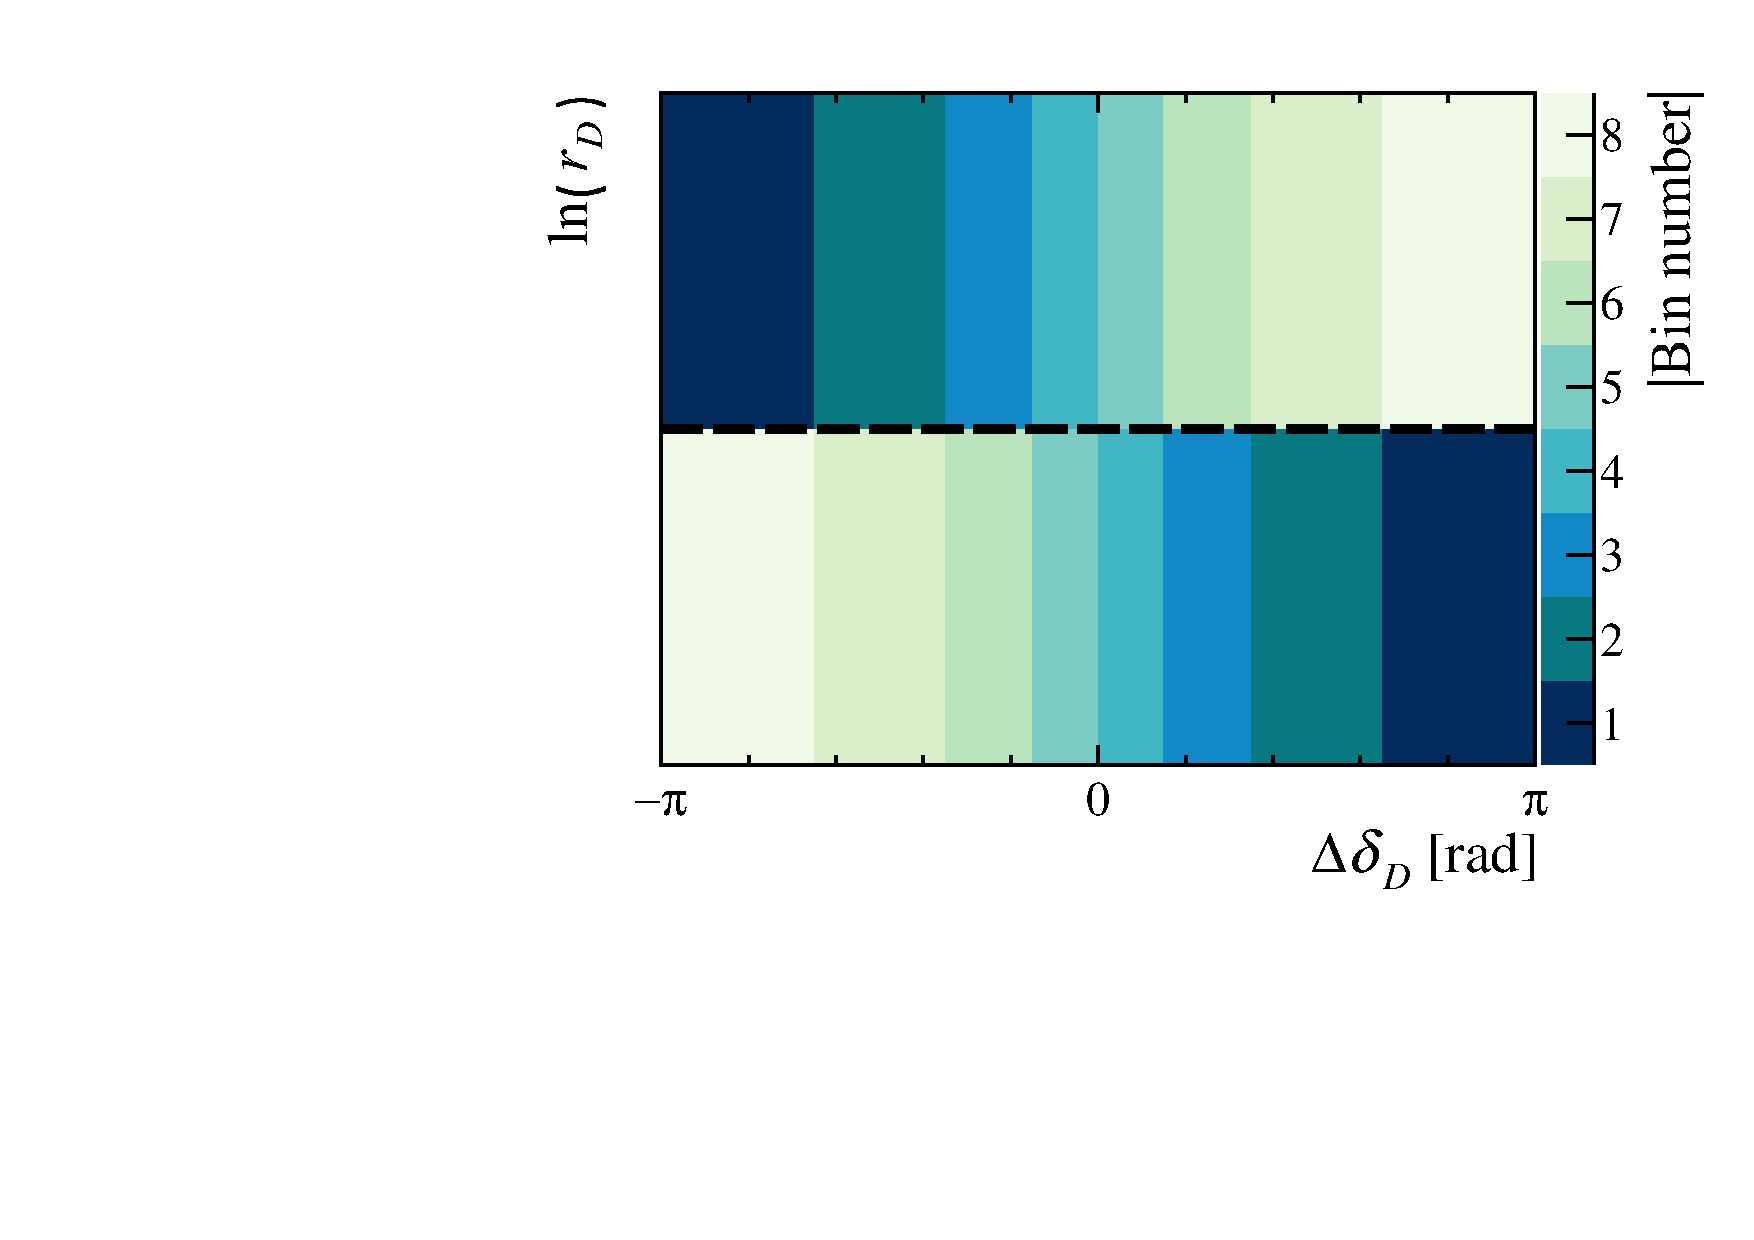
\includegraphics[width = 0.7\textwidth]{Plots/BinningSchemePlot_8Bins.pdf}
  \end{figure}
  \vspace{-1.0cm}
  \begin{center}
    $Q = 0.90$ \\
    Bins $i < 0$ on top, $i > 0$ below
  \end{center}
\end{frame}

\end{document}
